%% ============================================================
\clearpage
\section{Measurement Reliability: Variance Decomposition and Trial Count Justification}
\label{app:statistics}
%% ============================================================

\subsection{Variance decomposition}

Per-model metric scores reflect variance from scenario difficulty, trial stochasticity, and LLM judge stochasticity. We characterized the contributions of each on a subset of $N=4$ model configurations (2~cascade, 2~speech-to-speech) using 5~trials per scenario and 3~judge iterations per trial, across all 213 scenarios and 3~task domains. Three per-metric analyses were conducted: mixed effects variance decomposition (REML), two-way random effects ICC including the model $\times$ scenario interaction, and a permutation-based comparison of judge and trial standard deviations. Full results are reported below.

\paragraph{Mixed effects modelling.} We conducted variance decomposition using linear mixed effects modeling (REML), fitted separately within each model, with domain as a fixed effect and scenario and trial as nested random effects. For judge-graded metrics, judge iterations were included as an additional nested random effect; for deterministic metrics, trial is the lowest modeled level. In both cases, variance at the lowest level of the hierarchy is absorbed into the residual, as it cannot be separately identified without repeated observations at that level.

Trial was consistently the largest source of variance across all models, contributing 40-80\% of total observed variance for judge-graded metrics and 53-100\% for deterministic metrics. Trial variance exceeded scenario variance on all 9 metrics (33/34 model-metric combinations); across metrics, cross-model ranges of trial and scenario components did not overlap with the exception of a single-model, 1.5 point overlap for faithfulness (see \autoref{tab:LMM} for full decomposition). 

Scenario-level intraclass correlation (ICC), estimated as the proportion of total variance attributable to scenario identity, ranged from near zero to 47\% across metrics and models; \metrictaskcompletion~(ICC 33--47\% across models) and \metricfaithfulness~(ICC 21-42\%) showed consistently the highest scenario contributions. This is consistent with our observations that \metrictaskcompletion~and \metricfaithfulness~are inherently sensitive to intrinsic scenario difficulty, based in part on varying complexity of invoked policies.

%\input{figures/stats/tab_LMM}
\begingroup\small
\begin{longtable}{>{\raggedright\arraybackslash}p{2cm}lrrrr}
\caption{Per-model variance decomposition from REML linear mixed-effects fits with domain as a fixed effect and scenario and trial as nested random effects. For judge-graded metrics, judge iterations are an additional nested random effect, captured here in the \textit{Judge (\%)} column (the residual at the lowest level of the hierarchy). For deterministic metrics, trial is the lowest modeled level, so the \textit{Trial (\%)} column already absorbs the lowest-level variance and \textit{Judge (\%)} is left blank. All component columns give the proportion of total variance attributable to each component (\% of $\sigma^2_\text{total}$). Judge-graded metrics appear first, followed by deterministic metrics.}
\label{tab:LMM} \\
\toprule
Metric & Model & Scenario (\%) & Trial (\%) & Judge (\%) & $\sigma^2_\text{total}$ \\
\midrule
\endfirsthead
\multicolumn{6}{l}{\emph{Table~\ref{tab:LMM} continued from previous page}} \\
\toprule
Metric & Model & Scenario (\%) & Trial (\%) & Judge (\%) & $\sigma^2_\text{total}$ \\
\midrule
\endhead
\midrule \multicolumn{6}{r}{\emph{continued on next page}} \\
\endfoot
\bottomrule
\endlastfoot
Conciseness & \geminilive & 22.6 & 47.1 & 30.4 & 0.0114 \\
 & \gptrealtime & 26.4 & 42.0 & 31.6 & 0.0081 \\
 & \ink~+ \haiku~+ \sonic & 7.8 & 56.7 & 35.6 & 0.0090 \\
 & \parakeet~+ \gemmaB~+ \kokoro & 20.0 & 42.5 & 37.5 & 0.0076 \\
\midrule
Conversation progression & \geminilive & 20.9 & 56.0 & 23.2 & 0.1186 \\
 & \gptrealtime & 19.0 & 54.4 & 26.6 & 0.1034 \\
 & \ink~+ \haiku~+ \sonic & 4.0 & 59.1 & 36.8 & 0.0991 \\
 & \parakeet~+ \gemmaB~+ \kokoro & 15.9 & 56.9 & 27.1 & 0.0923 \\
\midrule
Faithfulness & \geminilive & 36.4 & 49.1 & 14.5 & 0.0942 \\
 & \gptrealtime & 41.9 & 40.4 & 17.7 & 0.1159 \\
 & \ink~+ \haiku~+ \sonic & 20.9 & 65.1 & 14.0 & 0.1616 \\
 & \parakeet~+ \gemmaB~+ \kokoro & 33.2 & 46.3 & 20.6 & 0.1458 \\
\midrule
Speech fidelity & \geminilive & 4.6 & 80.4 & 15.0 & 0.0032 \\
 & \gptrealtime & 0.0 & 71.6 & 28.4 & 0.0022 \\
 & \ink~+ \haiku~+ \sonic & 3.4 & 79.0 & 17.6 & 0.0028 \\
 & \parakeet~+ \gemmaB~+ \kokoro & 21.1 & 69.4 & 9.5 & 0.0109 \\
\midrule
Transcription accuracy key entities & \ink~+ \haiku~+ \sonic & 26.1 & 68.4 & 5.5 & 0.0679 \\
 & \parakeet~+ \gemmaB~+ \kokoro & 19.7 & 72.0 & 8.2 & 0.0393 \\
\midrule
Authentication success & \geminilive & 30.3 & 69.7 & -- & 0.1031 \\
 & \gptrealtime & 12.1 & 87.9 & -- & 0.0515 \\
 & \ink~+ \haiku~+ \sonic & 26.2 & 73.8 & -- & 0.2141 \\
 & \parakeet~+ \gemmaB~+ \kokoro & 24.8 & 75.2 & -- & 0.1090 \\
\midrule
Conversation completion & \geminilive & 0.0 & 100.0 & -- & 0.0431 \\
 & \gptrealtime & 2.1 & 97.9 & -- & 0.0139 \\
 & \ink~+ \haiku~+ \sonic & 14.9 & 85.1 & -- & 0.2025 \\
 & \parakeet~+ \gemmaB~+ \kokoro & 1.1 & 98.9 & -- & 0.0247 \\
\midrule
Task completion & \geminilive & 41.7 & 58.3 & -- & 0.2490 \\
 & \gptrealtime & 42.4 & 57.6 & -- & 0.1629 \\
 & \ink~+ \haiku~+ \sonic & 33.2 & 66.8 & -- & 0.2307 \\
 & \parakeet~+ \gemmaB~+ \kokoro & 47.3 & 52.7 & -- & 0.2333 \\
\midrule
Turn taking & \geminilive & 7.1 & 92.9 & -- & 0.0508 \\
 & \gptrealtime & 15.0 & 85.0 & -- & 0.0277 \\
 & \ink~+ \haiku~+ \sonic & 18.5 & 81.5 & -- & 0.0646 \\
 & \parakeet~+ \gemmaB~+ \kokoro & 21.6 & 78.4 & -- & 0.0267 \\
\end{longtable}
\endgroup

\paragraph{Scenario variance and model $\times$ scenario interaction.} To complement the full variance decomposition and assess whether models rank scenarios consistently, we computed two ICC models: a one-way ANOVA on model-centered scores, and a two-way random effects model including the model $\times$ scenario interaction term. The analysis covered eight metrics - authentication success, \metricconcise, \metricconversationcompletion, \metricconversationprogression, \metrictaskcompletion, \metrictranscription~(cascade-only), and \metricturntaking~- across the three task domains (CSM, ITSM, HR), yielding 22 domain $\times$ metric combinations. For each, we decomposed score variance into four components: scenario, model, model $\times$ scenario interaction, and residual trial-to-trial noise; variance components were estimated from a balanced two-way ANOVA. Significance was assessed via F-tests using the interaction mean square as the denominator (Cornfield-Tukey rule for random effects), and ICC$_\text{scenario}$ was reported as $\sigma^2_\text{scenario} / \sigma^2_\text{total}$. 

Per-metric scenario-level intraclass correlation (ICC$_{\text{scenario}}$, computed via one-way ANOVA after centering scores by model) ranged from approximately $0$ on metrics that saturate across most scenarios (\metricfidelity, \metricvalidend, \metricturntaking)~up to $0.31$ on \metrictaskcompletion~(see \autoref{tab:icc-pooled}). \metricfaithfulness~ranged $0.17$--$0.25$ across domains, \metricconcise~$0.12$--$0.13$, and \metricconversationprogression~$0.07$--$0.13$ . 

The model $\times$ scenario interaction was significant in all 22 domain $\times$ metric combinations ($p < 0.01$ in every case; $p < 0.001$ for 19 of 22; see \autoref{tab:icc-interaction}), accounting for 4–18\% of total score variance (median 11\%). This indicates that scenario difficulty is ranked differently across models; some scenarios are disproportionately harder for one model than another. Consistent with this finding, ICC$_\text{scenario}$ was low across the board (median 0.08, range 0.00–0.27), confirming that scenario identity alone explains a small fraction of overall score variance after accounting for model and interaction effects.

These analyses support the finding from the full variance decomposition that scenario is not the dominant source of variance, and is a property of the benchmark rather than a confound: it reflects the range of task difficulty that the benchmark spans. Additionally, this also demonstrates that a substantial proportion of each model's apparent scenario variance reflects model-specific scenario interactions rather than shared scenario difficulty.

\begingroup\footnotesize
\begin{longtable}{>{\raggedright\arraybackslash}p{1.8cm}lrrr}
\caption{Per-(metric $\times$ domain) scenario-level ICC from one-way ANOVA on per-model-centered scores. ICC$_\text{scenario}$ = $\sigma^2_\text{scenario} / (\sigma^2_\text{scenario} + \sigma^2_\text{residual})$. 95\% CI from the F-distribution (Fisher's exact ICC bounds). $n$ is the number of scenarios in the (metric, domain) cell.}
\label{tab:icc-pooled} \\
\toprule
Metric & Domain & ICC$_\text{scenario}$ & 95\% CI & $n$ \\
\midrule
\endfirsthead
\multicolumn{5}{l}{\emph{Table~\ref{tab:icc-pooled} continued from previous page}} \\
\toprule
Metric & Domain & ICC$_\text{scenario}$ & 95\% CI & $n$ \\
\midrule
\endhead
\midrule \multicolumn{5}{r}{\emph{continued on next page}} \\
\endfoot
\bottomrule
\endlastfoot
Authentication success & CSM & 0.112 & [0.066, 0.186] & 48 \\
 & ITSM & 0.065 & [0.037, 0.106] & 80 \\
 & HR & 0.214 & [0.160, 0.288] & 82 \\
\midrule
Conciseness & CSM & 0.132 & [0.082, 0.210] & 50 \\
 & ITSM & 0.115 & [0.077, 0.170] & 80 \\
 & HR & 0.129 & [0.089, 0.185] & 83 \\
\midrule
Conversation Completion & CSM & 0.002 & [0.000, 0.030] & 50 \\
 & ITSM & 0.019 & [0.002, 0.046] & 80 \\
 & HR & 0.041 & [0.019, 0.075] & 83 \\
\midrule
Conversation progression & CSM & 0.111 & [0.066, 0.183] & 50 \\
 & ITSM & 0.126 & [0.086, 0.183] & 80 \\
 & HR & 0.072 & [0.043, 0.114] & 83 \\
\midrule
Faithfulness & CSM & 0.247 & [0.174, 0.351] & 50 \\
 & ITSM & 0.173 & [0.110, 0.257] & 80 \\
 & HR & 0.231 & [0.174, 0.306] & 83 \\
\midrule
Speech fidelity & CSM & 0.017 & [0.000, 0.067] & 50 \\
 & ITSM & 0.020 & [0.001, 0.048] & 80 \\
 & HR & 0.000 & [0.000, 0.023] & 83 \\
\midrule
Task completion & CSM & 0.309 & [0.226, 0.421] & 50 \\
 & ITSM & 0.273 & [0.210, 0.355] & 80 \\
 & HR & 0.285 & [0.222, 0.367] & 83 \\
\midrule
Transcription accuracy key entities & CSM & 0.197 & [0.119, 0.308] & 50 \\
 & ITSM & 0.116 & [0.066, 0.187] & 80 \\
 & HR & 0.131 & [0.075, 0.205] & 83 \\
\midrule
Turn-taking & CSM & 0.040 & [0.013, 0.086] & 50 \\
 & ITSM & 0.051 & [0.027, 0.088] & 80 \\
 & HR & 0.020 & [0.002, 0.046] & 83 \\
\end{longtable}
\endgroup
\begingroup\footnotesize
\begin{longtable}{>{\raggedright\arraybackslash}p{1.8cm}lrrrrrr}
\caption{Per-(metric $\times$ domain) variance decomposition from a two-way random-effects ANOVA. Each row partitions total observed variance into scenario, model, model $\times$ scenario interaction, and residual components (\% of $\sigma^2_\text{total}$). $F_\text{int}$ and $p_\text{int}$ are the F-statistic and p-value for the interaction term, computed using the interaction mean square as the F-test denominator (Cornfield-Tukey rule for random effects).}
\label{tab:icc-interaction} \\
\toprule
Metric & Domain & Scenario (\%) & Model (\%) & Interaction (\%) & Residual (\%) & $F_\text{int}$ & $p_\text{int}$ \\
\midrule
\endfirsthead
\multicolumn{8}{l}{\emph{Table~\ref{tab:icc-interaction} continued from previous page}} \\
\toprule
Metric & Domain & Scenario (\%) & Model (\%) & Interaction (\%) & Residual (\%) & $F_\text{int}$ & $p_\text{int}$ \\
\midrule
\endhead
\midrule \multicolumn{8}{r}{\emph{continued on next page}} \\
\endfoot
\bottomrule
\endlastfoot
Authentication success & CSM & 9.7 & 1.0 & 6.4 & 83.0 & 1.38 & 0.004 \\
 & ITSM & 3.6 & 23.9 & 6.4 & 66.1 & 1.48 & $< 0.0001$ \\
 & HR & 14.7 & 18.7 & 12.5 & 54.0 & 2.16 & $< 0.0001$ \\
\midrule
Conciseness & CSM & 7.7 & 13.2 & 17.2 & 61.9 & 2.39 & $< 0.0001$ \\
 & ITSM & 8.0 & 1.1 & 16.1 & 74.9 & 2.07 & $< 0.0001$ \\
 & HR & 10.0 & 3.3 & 11.6 & 75.1 & 1.77 & $< 0.0001$ \\
\midrule
Conversation Completion & CSM & 0.0 & 2.1 & 8.0 & 89.9 & 1.44 & 0.001 \\
 & ITSM & 0.4 & 25.9 & 4.6 & 69.0 & 1.34 & 0.001 \\
 & HR & 0.6 & 44.3 & 8.1 & 47.0 & 1.86 & $< 0.0001$ \\
\midrule
Conversation progression & CSM & 8.3 & 6.7 & 9.5 & 75.5 & 1.63 & $< 0.0001$ \\
 & ITSM & 10.0 & 4.4 & 9.3 & 76.3 & 1.61 & $< 0.0001$ \\
 & HR & 4.2 & 5.1 & 12.3 & 78.4 & 1.78 & $< 0.0001$ \\
\midrule
Faithfulness & CSM & 20.7 & 6.2 & 10.9 & 62.1 & 1.88 & $< 0.0001$ \\
 & HR & 11.6 & 36.6 & 14.0 & 37.8 & 2.85 & $< 0.0001$ \\
\midrule
Task completion & CSM & 27.3 & 3.3 & 11.5 & 57.9 & 1.99 & $< 0.0001$ \\
 & ITSM & 18.6 & 20.5 & 14.3 & 46.6 & 2.53 & $< 0.0001$ \\
 & HR & 20.9 & 16.0 & 13.9 & 49.1 & 2.42 & $< 0.0001$ \\
\midrule
Transcription accuracy key entities & CSM & 7.3 & 21.1 & 18.3 & 53.3 & 2.71 & $< 0.0001$ \\
 & ITSM & 2.9 & 20.8 & 14.2 & 62.1 & 2.14 & $< 0.0001$ \\
\midrule
Turn taking & CSM & 0.6 & 63.2 & 4.2 & 32.0 & 1.66 & $< 0.0001$ \\
 & ITSM & 0.8 & 65.6 & 4.7 & 29.0 & 1.81 & $< 0.0001$ \\
 & HR & 0.0 & 73.0 & 4.5 & 22.5 & 2.01 & $< 0.0001$ \\
\end{longtable}
\endgroup

\paragraph{Judge stochasticity.} We assessed whether trial standard deviation systematically exceeds judge standard deviation using a sign-flip permutation test on the mean delta (trial SD - judge SD delta per scenario, within or averaged across models; one-sided, $H_1$: mean delta > 0; 10,000 permutations). As a complementary check on directional consistency, we applied an exact binomial sign test to the count of scenarios where the delta exceeded zero (one-sided, $H_1$: $P(delta > 0) > 0.5$). 

Trial variance dominated judge variance across all 16 model $\times$ metric combinations (sign-flip permutation test, one-sided, $p < 0.0001$ in every case; see \autoref{tab:judge-trial}, with per-model mean deltas between trial and judge standard deviations ranging from 0.01–0.05 for agent's \metricfidelity~and 0.02–0.03 for \metricconcise, to 0.12–0.15 for \metricconversationprogression~and 0.11–0.21 for \metricfaithfulness. The binomial sign test confirmed that trial SD exceeded judge SD in the majority of scenarios for 13 of 16 model $\times$ metric combinations ($p < 0.05$). For 3 models, the significant mean deltas for agent \metricfidelity, which had negligible variance for both judge and trial, were driven by a minority of high-variance scenarios or a p-value just above the threshold.

\begingroup\footnotesize
\begin{longtable}{
%>{\raggedright\arraybackslash}p{1.8cm}llrrrr}
  >{\raggedright\arraybackslash}p{1.2cm}
  >{\raggedright\arraybackslash}p{1.0cm}
  >{\raggedright\arraybackslash}p{3.8cm}
  >{\centering\arraybackslash}p{1.4cm}
  >{\centering\arraybackslash}p{1.4cm}
  >{\centering\arraybackslash}p{1.4cm}
  >{\centering\arraybackslash}p{1.4cm}}
\caption{Judge vs. trial variance per domain and model. Each cell value is the mean across records of the per-record standard deviation: \textit{Judge std dev} is the per-record SD across the 3 judge iterations (averaged over trials before averaging across records); \textit{Trial std dev} is the per-record SD across trials (after averaging across judge iterations), averaged across records. $p_\text{perm}$ is the one-sided sign-flip permutation test p-value (10,000 permutations, $H_1$: trial std dev $>$ judge std dev). $p_\text{sign}$ is the one-sided exact binomial sign test p-value ($H_1$: P(trial std dev $>$ judge std dev) $> 0.5$).}
\label{tab:judge-trial} \\
\toprule
Metric & Domain & Model & Judge std dev & Trial std dev & $p_\text{perm}$ & $p_\text{sign}$ \\
\midrule
\endfirsthead
\multicolumn{7}{l}{\emph{Table~\ref{tab:judge-trial} continued from previous page}} \\
\toprule
Metric & Domain & Model & Judge std dev & Trial std dev & $p_\text{perm}$ & $p_\text{sign}$ \\
\midrule
\endhead
\midrule \multicolumn{7}{r}{\emph{continued on next page}} \\
\endfoot
\bottomrule
\endlastfoot
Conciseness & CSM & \geminilive & 0.0364 & 0.0681 & $< 0.0001$ & $< 0.0001$ \\
 & CSM & \parakeet~+ \gemmaB~+ \kokoro & 0.0401 & 0.0489 & 0.004 & 0.003 \\
 & CSM & \gptrealtime & 0.0345 & 0.0649 & $< 0.0001$ & $< 0.0001$ \\
 & CSM & \ink~+ \haiku~+ \sonic & 0.0412 & 0.0665 & $< 0.0001$ & $< 0.0001$ \\
 & ITSM & \geminilive & 0.0367 & 0.0684 & $< 0.0001$ & $< 0.0001$ \\
 & ITSM & \parakeet~+ \gemmaB~+ \kokoro & 0.0349 & 0.0522 & $< 0.0001$ & $< 0.0001$ \\
 & ITSM & \gptrealtime & 0.0311 & 0.0529 & $< 0.0001$ & $< 0.0001$ \\
 & ITSM & \ink~+ \haiku~+ \sonic & 0.0370 & 0.0645 & $< 0.0001$ & $< 0.0001$ \\
 & HR & \geminilive & 0.0386 & 0.0651 & $< 0.0001$ & $< 0.0001$ \\
 & HR & \parakeet~+ \gemmaB~+ \kokoro & 0.0325 & 0.0547 & $< 0.0001$ & $< 0.0001$ \\
 & HR & \gptrealtime & 0.0319 & 0.0473 & $< 0.0001$ & $< 0.0001$ \\
 & HR & \ink~+ \haiku~+ \sonic & 0.0382 & 0.0648 & $< 0.0001$ & $< 0.0001$ \\
\midrule
Conversation progression & CSM & \geminilive & 0.0535 & 0.2259 & $< 0.0001$ & $< 0.0001$ \\
 & CSM & \parakeet~+ \gemmaB~+ \kokoro & 0.0639 & 0.1417 & $< 0.0001$ & 0.008 \\
 & CSM & \gptrealtime & 0.0655 & 0.2303 & $< 0.0001$ & $< 0.0001$ \\
 & CSM & \ink~+ \haiku~+ \sonic & 0.0960 & 0.2048 & $< 0.0001$ & $< 0.0001$ \\
 & ITSM & \geminilive & 0.0735 & 0.2184 & $< 0.0001$ & $< 0.0001$ \\
 & ITSM & \parakeet~+ \gemmaB~+ \kokoro & 0.0631 & 0.1823 & $< 0.0001$ & $< 0.0001$ \\
 & ITSM & \gptrealtime & 0.0726 & 0.2003 & $< 0.0001$ & $< 0.0001$ \\
 & ITSM & \ink~+ \haiku~+ \sonic & 0.0901 & 0.2301 & $< 0.0001$ & $< 0.0001$ \\
 & HR & \geminilive & 0.0840 & 0.2287 & $< 0.0001$ & $< 0.0001$ \\
 & HR & \parakeet~+ \gemmaB~+ \kokoro & 0.0762 & 0.2257 & $< 0.0001$ & $< 0.0001$ \\
 & HR & \gptrealtime & 0.0799 & 0.2056 & $< 0.0001$ & $< 0.0001$ \\
 & HR & \ink~+ \haiku~+ \sonic & 0.0850 & 0.2206 & $< 0.0001$ & $< 0.0001$ \\
\midrule
Faithfulness & CSM & \geminilive & 0.0532 & 0.2519 & $< 0.0001$ & $< 0.0001$ \\
 & CSM & \parakeet~+ \gemmaB~+ \kokoro & 0.0749 & 0.2621 & $< 0.0001$ & $< 0.001$ \\
 & CSM & \gptrealtime & 0.0532 & 0.2145 & $< 0.0001$ & $< 0.0001$ \\
 & CSM & \ink~+ \haiku~+ \sonic & 0.0666 & 0.2869 & $< 0.0001$ & $< 0.0001$ \\
 & ITSM & \geminilive & 0.0303 & 0.1295 & $< 0.0001$ & 0.073 \\
 & ITSM & \parakeet~+ \gemmaB~+ \kokoro & 0.0869 & 0.1853 & $< 0.0001$ & $< 0.0001$ \\
 & ITSM & \gptrealtime & 0.0693 & 0.1782 & $< 0.0001$ & $< 0.0001$ \\
 & ITSM & \ink~+ \haiku~+ \sonic & 0.0564 & 0.2767 & $< 0.0001$ & $< 0.0001$ \\
 & HR & \geminilive & 0.0307 & 0.1001 & $< 0.0001$ & 0.745 \\
 & HR & \parakeet~+ \gemmaB~+ \kokoro & 0.0763 & 0.2091 & $< 0.0001$ & $< 0.0001$ \\
 & HR & \gptrealtime & 0.0426 & 0.1287 & $< 0.0001$ & 0.008 \\
 & HR & \ink~+ \haiku~+ \sonic & 0.0548 & 0.2517 & $< 0.0001$ & $< 0.0001$ \\
\midrule
Speech fidelity & CSM & \geminilive & 0.0000 & 0.0000 & 0.500 & 1.000 \\
 & CSM & \parakeet~+ \gemmaB~+ \kokoro & 0.0044 & 0.0425 & $< 0.0001$ & 0.899 \\
 & CSM & \gptrealtime & 0.0027 & 0.0158 & 0.033 & 1.000 \\
 & CSM & \ink~+ \haiku~+ \sonic & 0.0020 & 0.0148 & $< 0.0001$ & 0.984 \\
 & ITSM & \geminilive & 0.0047 & 0.0314 & $< 0.0001$ & 1.000 \\
 & ITSM & \parakeet~+ \gemmaB~+ \kokoro & 0.0074 & 0.0559 & $< 0.0001$ & $< 0.0001$ \\
 & ITSM & \gptrealtime & 0.0020 & 0.0057 & 0.017 & 1.000 \\
 & ITSM & \ink~+ \haiku~+ \sonic & 0.0051 & 0.0353 & $< 0.0001$ & $< 0.001$ \\
 & HR & \geminilive & 0.0011 & 0.0044 & 0.032 & 1.000 \\
 & HR & \parakeet~+ \gemmaB~+ \kokoro & 0.0060 & 0.0598 & $< 0.0001$ & $< 0.0001$ \\
 & HR & \gptrealtime & 0.0013 & 0.0083 & $< 0.0001$ & 1.000 \\
 & HR & \ink~+ \haiku~+ \sonic & 0.0020 & 0.0284 & $< 0.0001$ & 0.413 \\
\midrule
Transcription accuracy key entities & CSM & \parakeet~+ \gemmaB~+ \kokoro & 0.0148 & 0.1316 & $< 0.0001$ & $< 0.0001$ \\
 & CSM & \ink~+ \haiku~+ \sonic & 0.0243 & 0.1685 & $< 0.0001$ & $< 0.0001$ \\
 & ITSM & \parakeet~+ \gemmaB~+ \kokoro & 0.0278 & 0.1261 & $< 0.0001$ & $< 0.0001$ \\
 & ITSM & \ink~+ \haiku~+ \sonic & 0.0204 & 0.1819 & $< 0.0001$ & $< 0.0001$ \\
 & HR & \parakeet~+ \gemmaB~+ \kokoro & 0.0250 & 0.1521 & $< 0.0001$ & $< 0.0001$ \\
 & HR & \ink~+ \haiku~+ \sonic & 0.0285 & 0.1875 & $< 0.0001$ & $< 0.0001$ \\
\end{longtable}
\endgroup
%\input{figures/stats/tab_judge-trial}
% \input{figures/stats/outdated_tab_wilcoxon_trial_vs_judge}

\subsection{Justification of trial count}
\label{app:trial_count}

\paragraph{Motivation.}
EVA-Bench averages over multiple trials per scenario to reduce
simulator and agent stochasticity. Clean evaluations use $k{=}5$
trials per scenario, while perturbation experiments use $k{=}3$ to
fit a larger cell count within compute budget. We quantify the cost of
this reduction by measuring how rapidly each model-level metric
estimate stabilizes as a function of trial count.

\paragraph{Method.}
For each (model, metric) pair and each $k \in \{1,2,3,4\}$ we draw
$N{=}2000$ Monte Carlo subsamples. In each draw, we independently
sample, for every scenario, a uniformly random $k$-trial subset of the
five available trials, average within scenario, then average across
scenarios. The result is a single model-level estimate
$\hat{\theta}_k$ per draw. At $k{=}5$ exactly one draw exists --
the {\em anchor} $\hat{\theta}_5$, equal to the full
mean-of-scenario-means.

We sample subsets {\em independently per scenario} rather than
aligning trial indices across scenarios, because trial indices are not
meaningful across scenarios.

For each $k$ we report the {\bf 95\% interval width}
        $w_k = p_{97.5}(\hat{\theta}_k) - p_{2.5}(\hat{\theta}_k)$,
        in metric units.

These quantities reflect resampling of {\em existing} trial
outcomes -- they capture how much our reported estimate would have
moved if we had used fewer of the trials we ran. The pooled bootstrap CIs in the main results (Sec.~\ref{sec:main-results}) capture the complementary cross-scenario uncertainty.

\paragraph{Results.}
Figure~\ref{fig:trial_count_ci} plots the median 95\% CI width at
each $k$, one panel per metric, one line per model. Every line decays
approximately as $k^{-1/2}$ -- the textbook scaling for sample-mean
variance -- with two regimes:

\begin{itemize}\itemsep0pt
  \item {\em Per-turn metrics} (\metricfidelity, \metricconcise,
        \metricturntaking) are already stable at $k{=}1$, with CI width
        below $0.02$ across all models. Adding trials yields little
        further reduction.
  \item {\em Conversation-level and pass metrics} (EVA-A pass@1, EVA-X pass@1, Task
        Completion, Faithfulness, Conversation Progression) are noisier: CI
        width is $0.05$--$0.09$ at $k{=}1$, shrinking to roughly
        $0.02$--$0.03$ at $k{=}3$.
\end{itemize}

Table~\ref{tab:trial_count_summary} summarises. At $k{=}3$, the
median 95\% CI width is at most 0.034 for any metric, and
at least 97.3\% of $k{=}3$ subsamples land within
$0.02$ of the $k{=}5$ anchor on every metric.

\paragraph{Justifying the trial counts.}
Cross-model gaps on the headline pass-style metrics span $0.1$--$0.6$
across the 12 evaluated systems. At $k{=}3$, trial-count uncertainty
is $\sim\!0.03$ -- below 10\% of the smallest interesting effect size
and well below the cross-architecture gaps reported in the main
tables. We therefore use $k{=}3$ for the perturbation experiments,
where holding the trial count down lets us cover more scenarios. We
retain $k{=}5$ for the clean evaluation, where the same point
estimates are reused across scatter plots and Pareto frontiers and
the marginal CI shrinkage from $k{=}4$ to $k{=}5$ ($\sim\!0.02$
absolute, by construction terminating at zero) is worth the cost.

\begin{figure}[h]
\centering
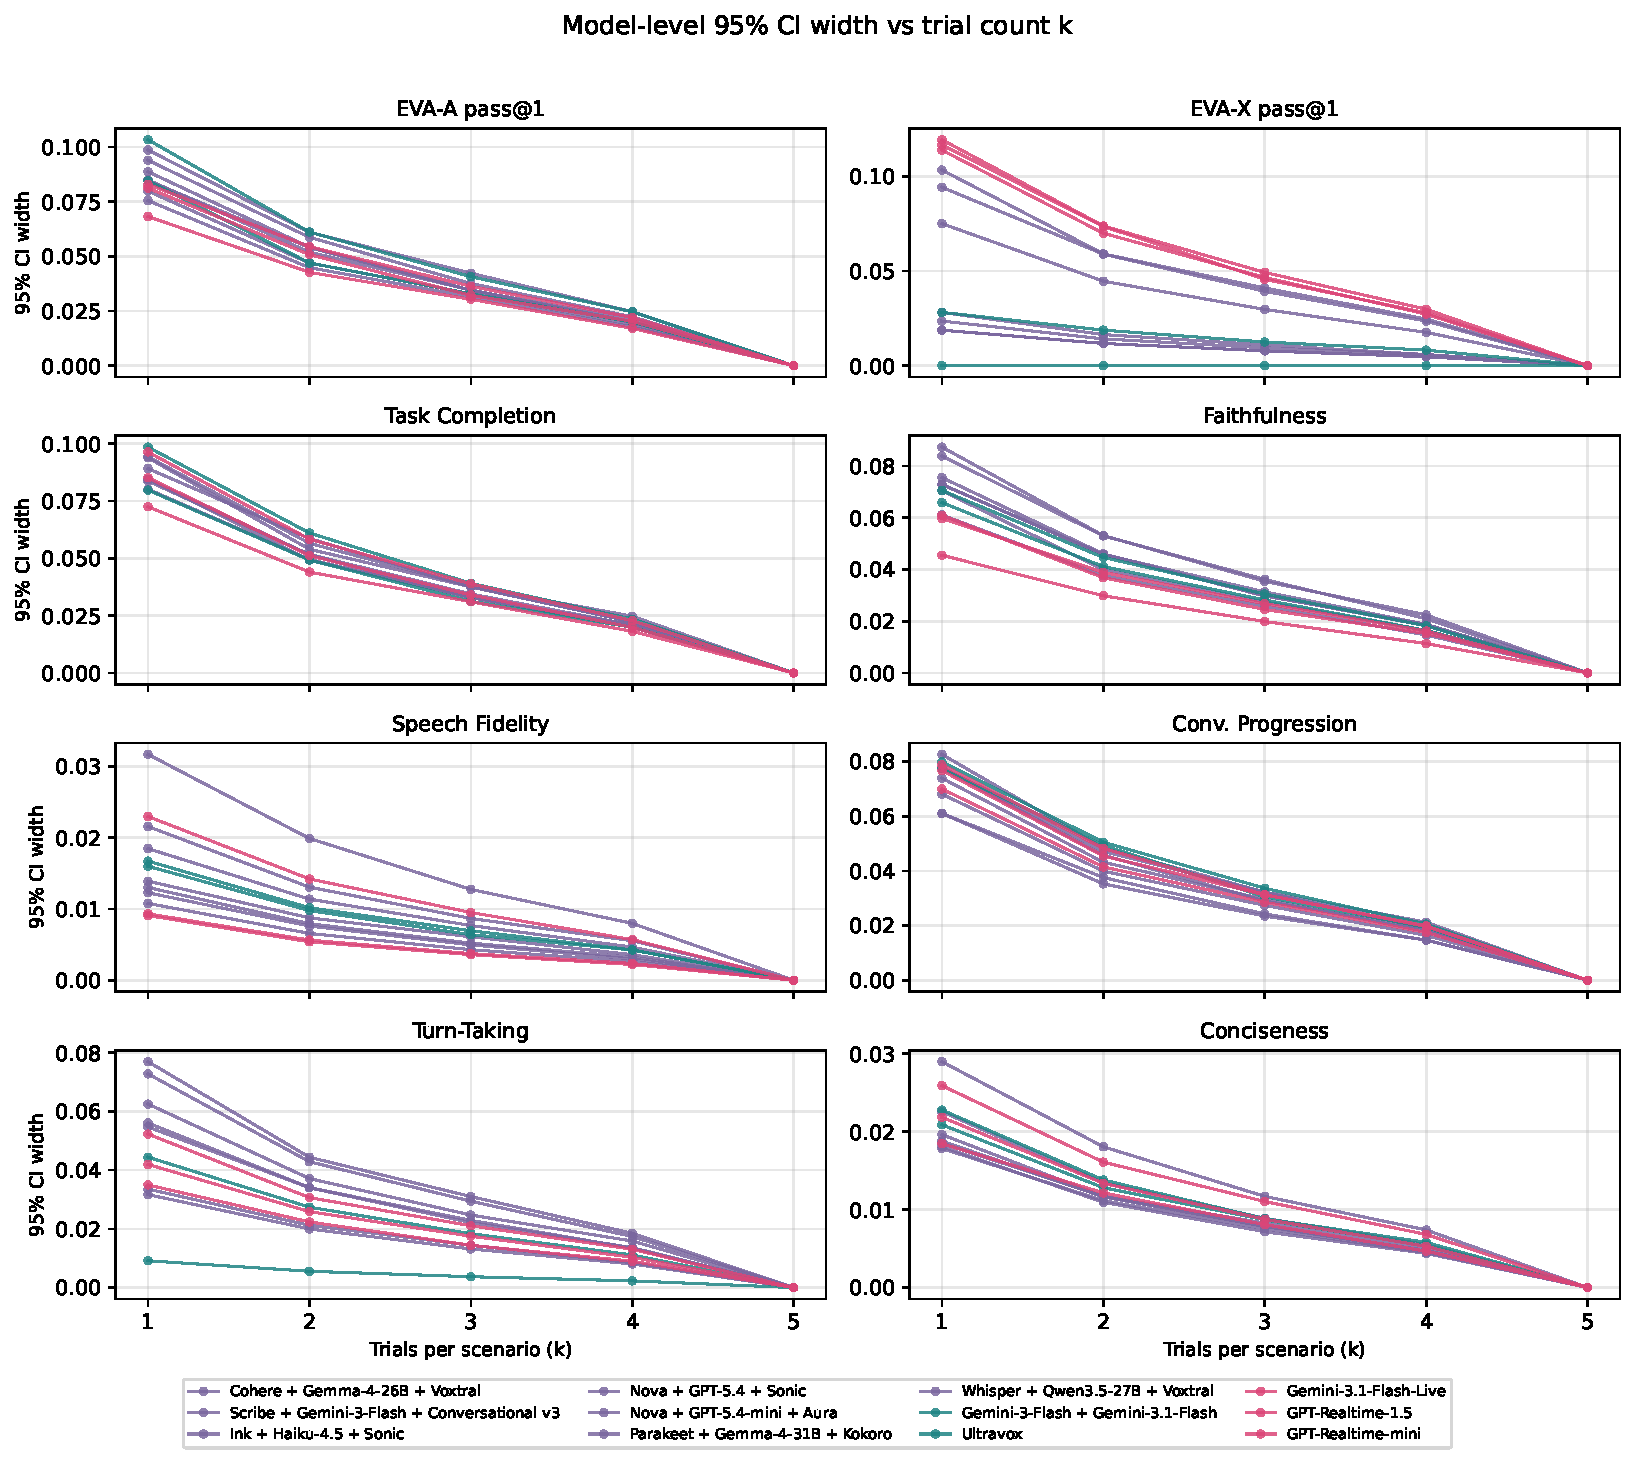
\includegraphics[width=\textwidth]{figures/trial_count/trial_count_grid_ci_width.pdf}
\caption{Model-level 95\% empirical CI width as a function of trial
count $k$, one panel per metric. Each line is one of the 12 evaluated
systems. Width is computed as $p_{97.5}-p_{2.5}$ over $N{=}2000$
Monte Carlo subsamples per $(model, metric, k)$. The $k{=}5$ point
is identically zero (single-anchor draw).}
\label{fig:trial_count_ci}
\end{figure}

\begin{table}[h]
\centering\small
\caption{Subsample-stability summary across the 12 evaluated systems.
\emph{Median 95\% CI width:} median across models of the empirical
$p_{97.5}{-}p_{2.5}$ width of the model-level estimate at trial count $k$,
in metric units. \emph{Agree $\le$0.02:} median across models of the
fraction of $k{=}3$ subsamples that fall within $0.02$ of the $k{=}5$
anchor. The $k{=}5$ column is omitted because it is identically zero by
construction (single anchor draw).}
\begin{tabular}{lccccc}
\toprule
\textbf{Metric} & \multicolumn{4}{c}{\textbf{Median 95\% CI width}} & \textbf{Agree $\le$0.02} \\
\cmidrule(lr){2-5} \cmidrule(lr){6-6}
 & $k{=}1$ & $k{=}2$ & $k{=}3$ & $k{=}4$ & at $k{=}3$ \\
\midrule
  EVA-A pass@1 & 0.085 & 0.053 & 0.034 & 0.020 & 97.6\% \\
  EVA-X pass@1 & 0.052 & 0.032 & 0.021 & 0.013 & 99.6\% \\
  Task Completion & 0.085 & 0.052 & 0.034 & 0.021 & 97.3\% \\
  Faithfulness & 0.070 & 0.043 & 0.029 & 0.017 & 99.4\% \\
  Speech Fidelity & 0.015 & 0.009 & 0.006 & 0.004 & 100.0\% \\
  Conv. Progression & 0.077 & 0.046 & 0.030 & 0.019 & 99.1\% \\
  Turn-Taking & 0.048 & 0.029 & 0.020 & 0.012 & 100.0\% \\
  Conciseness & 0.020 & 0.012 & 0.008 & 0.005 & 100.0\% \\
\bottomrule
\end{tabular}
\label{tab:trial_count_summary}
\end{table}
